\documentclass{article}
\usepackage[utf8]{inputenc}
\usepackage{polski}
\usepackage{graphicx}

\begin{titlepage}
    \title{FilterStudio Design Document}    
    \author{Paweł Chłąd \\ Bartłomiej Meller \\ Daniel Jambor }
\end{titlepage}


\begin{document}

\maketitle
\pagebreak


\section{Overview}

The following document covers overall design and features of FilterStudio application.

FilterStudio is a tool that allows users to design and test image filters. Users can 
design individual filters and also combine different filters together. 


\subsection{Features}


\begin{itemize}
\item \textbf{Filter Design} - Capability to construct basic matrix filters, user can specify
how big filter is and what values are used in it.

\item \textbf{Filter Project View} - Capability to join diffrent filters together, and manage
multiple filters as a one project.

\item \textbf{Filter and Filter Project Saving} - Capability to save filter and filter groups to file (prefably JSON)
\item \textbf{Live Image View} - Capability to load any image to the application that will allow users to see
how filter or filter group work on certain image. Any change to filter or filter group will refresh Live Image View to show
reflected changes.
\item \textbf{Image Saving} - Capability to save changed images 
\end{itemize}


\section{Detailed feature overview}
This section contains detailed feature descriptions

\subsection{Filter Design}
This feature allows users for designing basic matrix filters. Users can choose size of matrix in two dimensions, the view will resize accordingly to the size of a filter. Matrix View will consist of "tiles" in which you can write some integer value. After adjusting any value or size of the filter, Live Image View should update accordingly

\subsection{Filter Project View}
This feature allows users for desiging groups of filters. The order in which individual filters / operations are shown in this view reflects the order of execution of filters. The whole thing can be shown as a tree of filters or as a list (in simpler scenarion). On the top of the tree there is an special default input node, which simply just passes any input to the tree below.


\subsection{Filter and Filter Project Saving} 
This feature allows users for saving individual filters as well as whole filter project. Needed for users so that they can continue working after closing and opening the application.

\subsection{Live Image View}
This feature allows users for viewing last input and output of individual filter or filter group. This feature can be turned off to decrease amount of work that is done by processor. If Live View is turned on any change in group or in any individual filter in that group will trigger Live View update and the appropiate image will be shown.

\subsection{Image Saving}
This feature allows users to save individual images from filters or filter groups.

\newpage
\section{User's Manual}
This section provides information about usage of the FilterStudio application.

\subsection{Overview}

\bigskip
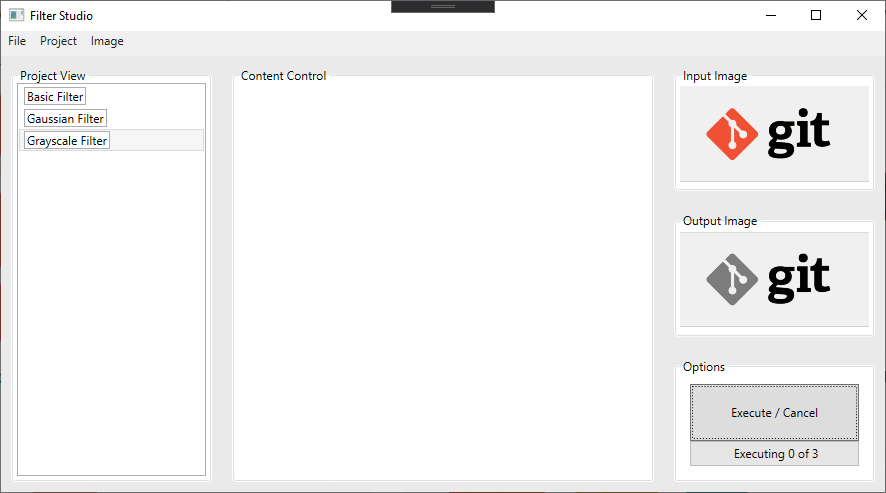
\includegraphics[width=0.9\textwidth]{overview.png}

\begin{itemize}
    \item \emph{Project View} -- Lists all active filters and allows user to navigate and edit them by clicking.
    \item \emph{Content Control} -- Alows user to edit filters, see "Gaussian Filter" and "Basic Matrix Filters" sections
    \item \emph{Input Image} -- Shows chosen input image thumbnail
    \item \emph{Output Image} -- Shows filtered image preview thumbnail
    \item \emph{Options} -- This section contains button that allows user to render filtered image and a progress indicator.
\end{itemize}

\newpage
\subsection{Gausian Filter}
To add Gaussian Filter to project click \textbf{Project $\rightarrow$ Add New Filter $\rightarrow$ Gaussian Filter},

\bigskip
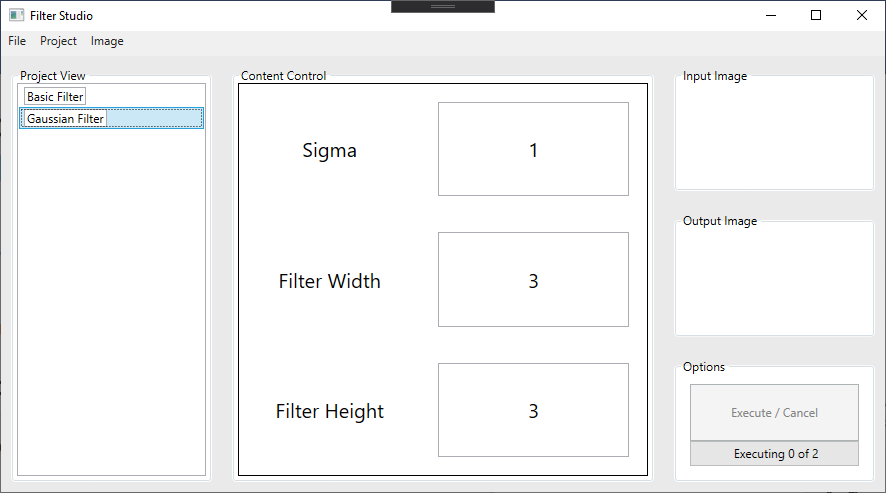
\includegraphics[width=0.9\textwidth]{gauss.png}
\bigskip

and enter parameters into appropriate textboxes.

\subsection{Basic Matrix Filter}
To add Gaussian Filter to project click \textbf{Project $\rightarrow$ Add New Filter $\rightarrow$ Basic Matrix Filter},

\bigskip
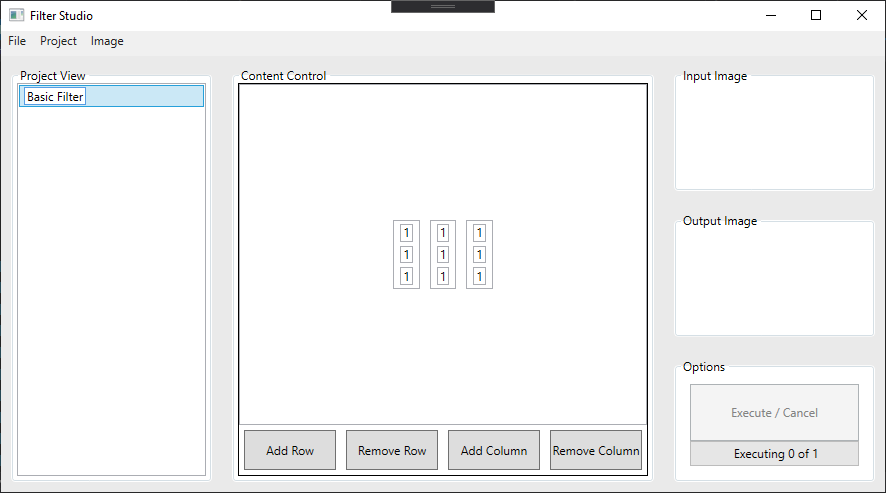
\includegraphics[width=0.9\textwidth]{matrix.png}
\bigskip

adjutst matrix dimmensions with buttons visible in bottom part of \textbf{Content Control} and enter values into cells.

\subsection{Greyscale Filter}
To add Gaussian Filter to project click \textbf{Project $\rightarrow$ Add New Filter $\rightarrow$ Greyscale Filter}

\subsection{Loading, saving and creating projects}
All this features are available in \textbf{File} menu and works in standard Windows manner.

\subsection{Loading and saving images}
Both features are available in \textbf{Image} menu and works in standard Windows manner.


\end{document}
